\documentclass[9pt]{beamer}
\mode<presentation>
\usepackage[T1]{fontenc}
\usepackage{color}
\usepackage{graphicx}
\usepackage{natbib}
\usepackage{tikz}
\usetikzlibrary{shapes.geometric}
\usepackage{xmpmulti}
\usepackage{animate}
\usepackage{tcolorbox}
\usepackage{amsmath}
\usepackage{gensymb}
\usepackage{csquotes}
\usepackage{bibentry}
\nobibliography*

\usetheme{Singapore}
%\usecolortheme{seahorse}

\usefonttheme{professionalfonts}

\title[Word \& Doc Embeddings]{A Rapid Computer-assisted Systematic Map of Regional Climate Impacts}
%\author{Max Callaghan, Gerritt }
\institute[MCC]{
	
\includegraphics[height=1cm,width=2cm]{images/MCC_Logo_RZ_rgb.jpg} \hspace{5em} 
\includegraphics[height=1cm]{images/climate_analytics.png}
}

\newif\ifframeinlbf
\frameinlbftrue
\makeatletter
\newcommand\listofframes{\@starttoc{lbf}}
\makeatother

\addtobeamertemplate{frametitle}{}{%
	\ifframeinlbf
	\addcontentsline{lbf}{section}{\protect\makebox[2em][l]{%
			\protect\usebeamercolor[fg]{structure}\insertframenumber\hfill}%
		\insertframetitle\par}%
	\else\fi
}

\newtheorem*{remark}{}

\bibliographystyle{apalike}

\begin{document}


\begin{frame}{In which locations is there evidence? What impacts does it document? Since when has there been evidence?}

\begin{columns}
	\begin{column}{0.382\linewidth}
		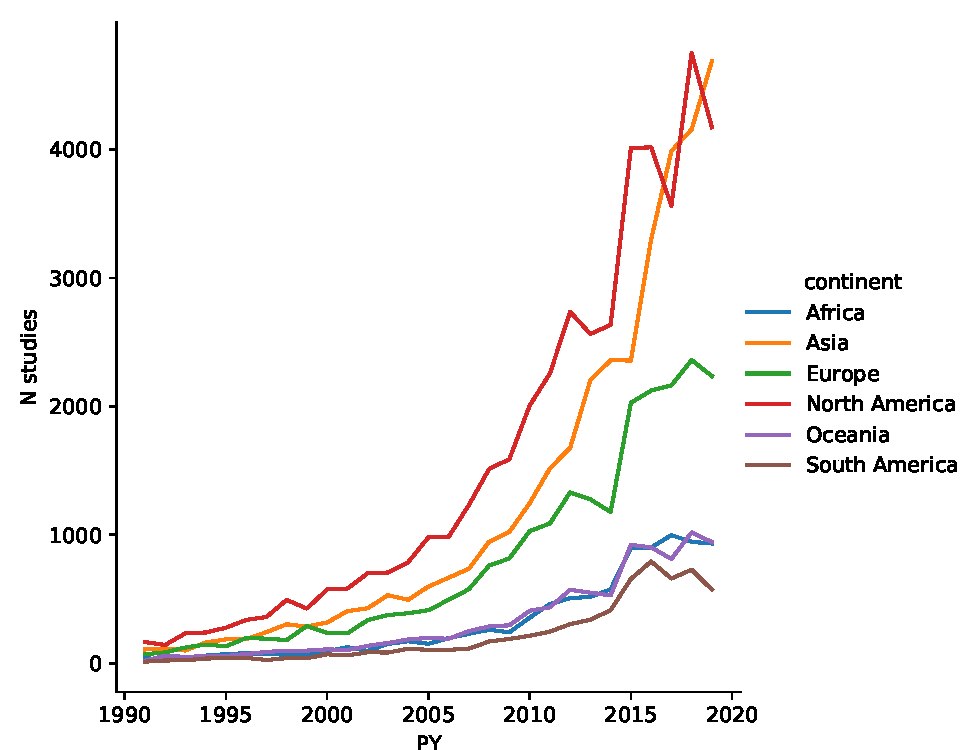
\includegraphics[width=\linewidth]{../plots/literature_distribution/PY_continent_n.pdf}
		
		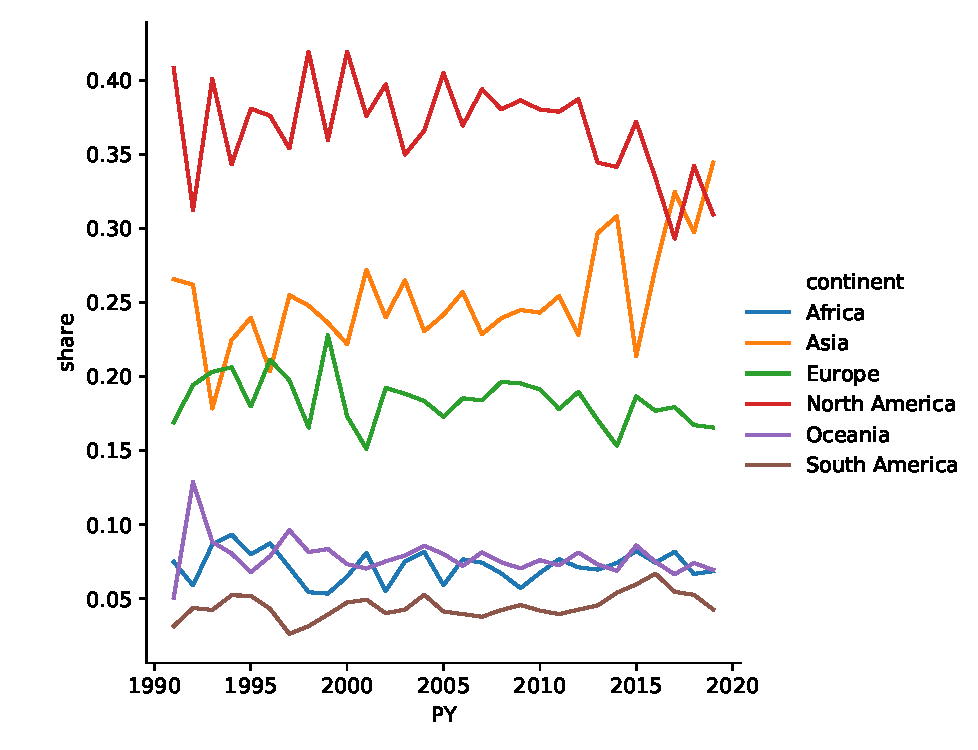
\includegraphics[width=\linewidth]{../plots/literature_distribution/PY_continent_shares.pdf}
	\end{column}
	\begin{column}{0.618\linewidth}
		\begin{itemize}
			\item More studies on Asia than North America since 2018
			\item Africa now more frequently studied than South America and Oceania
			
		\end{itemize}
	\end{column}
\end{columns}

\end{frame}

%%%

\begin{frame}{}

\begin{columns}
\begin{column}{0.382\linewidth}
	\begin{itemize}
		\item<1-> Lots of the new studies on Asia have been about Detection (is there a regional climate trend?)
		\item<2-> There is also more literature on human impacts and the water cycle in Asia
		\item<3-> On human impacts, Africa is as much studied as anywhere apart from Asia
		
	\end{itemize}
\end{column}
\begin{column}{0.618\linewidth}
	\only<1->{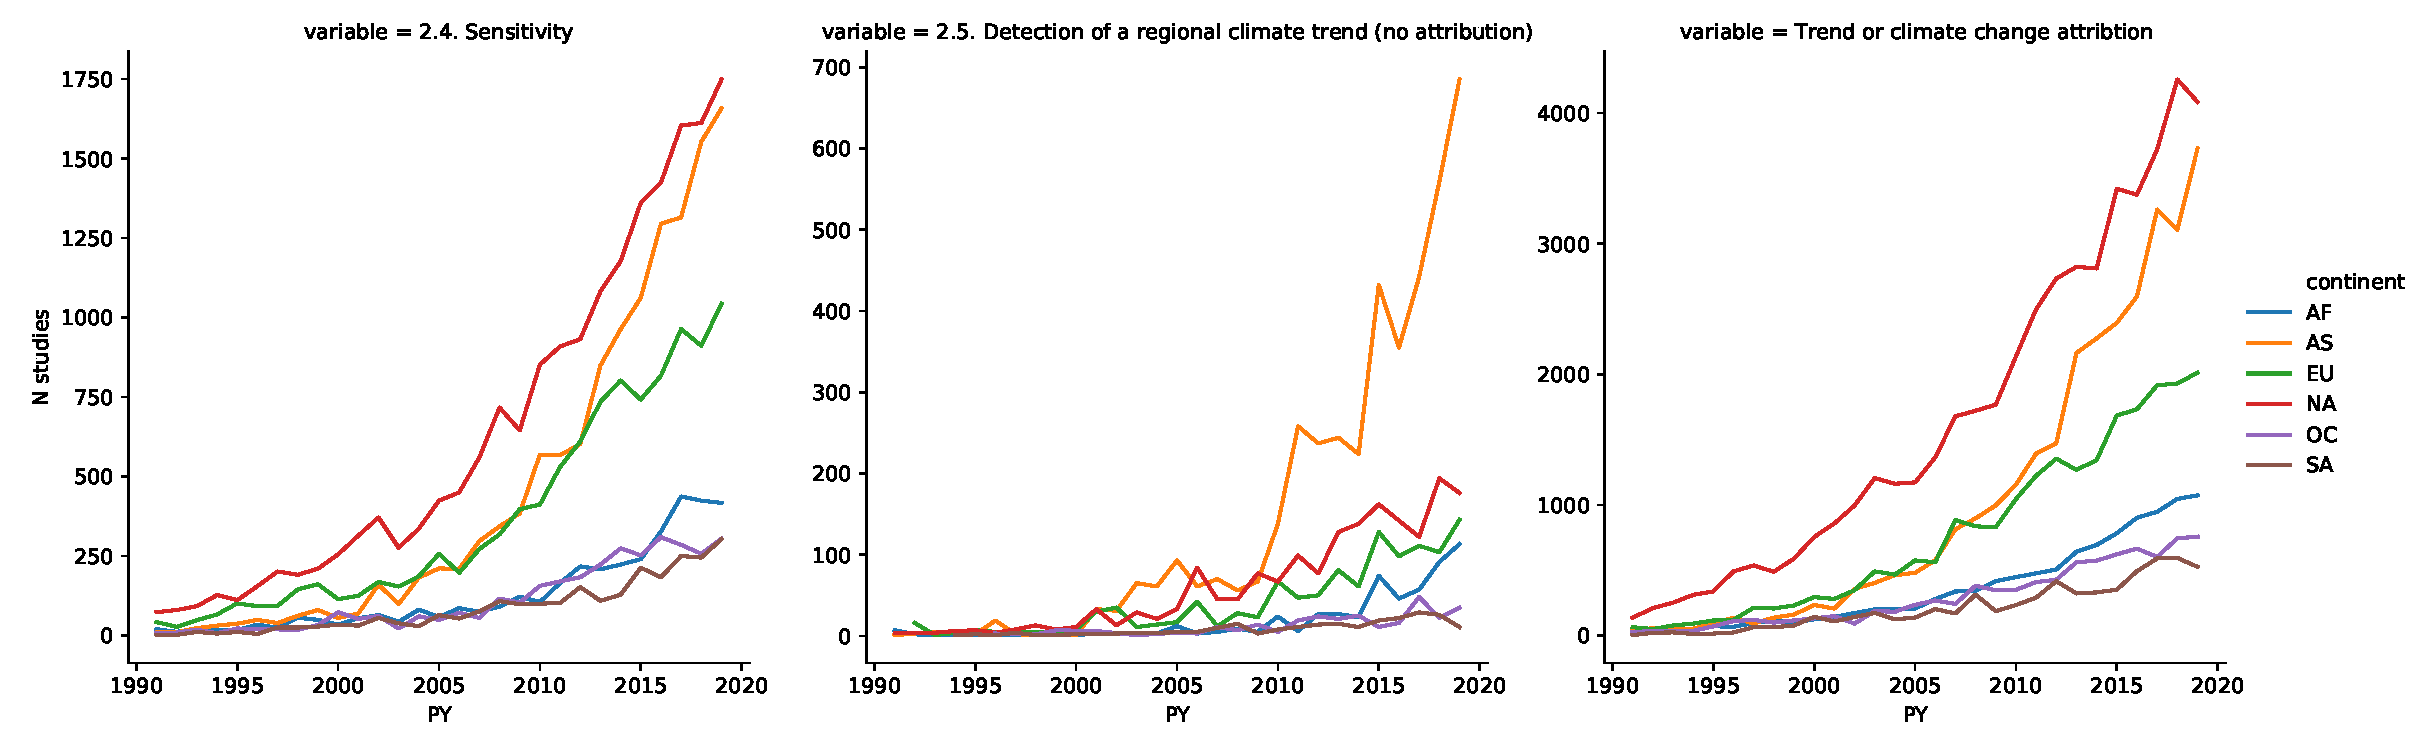
\includegraphics[width=\linewidth]{../plots/literature_distribution/PY_continent_attrib.pdf}}
	\only<2->{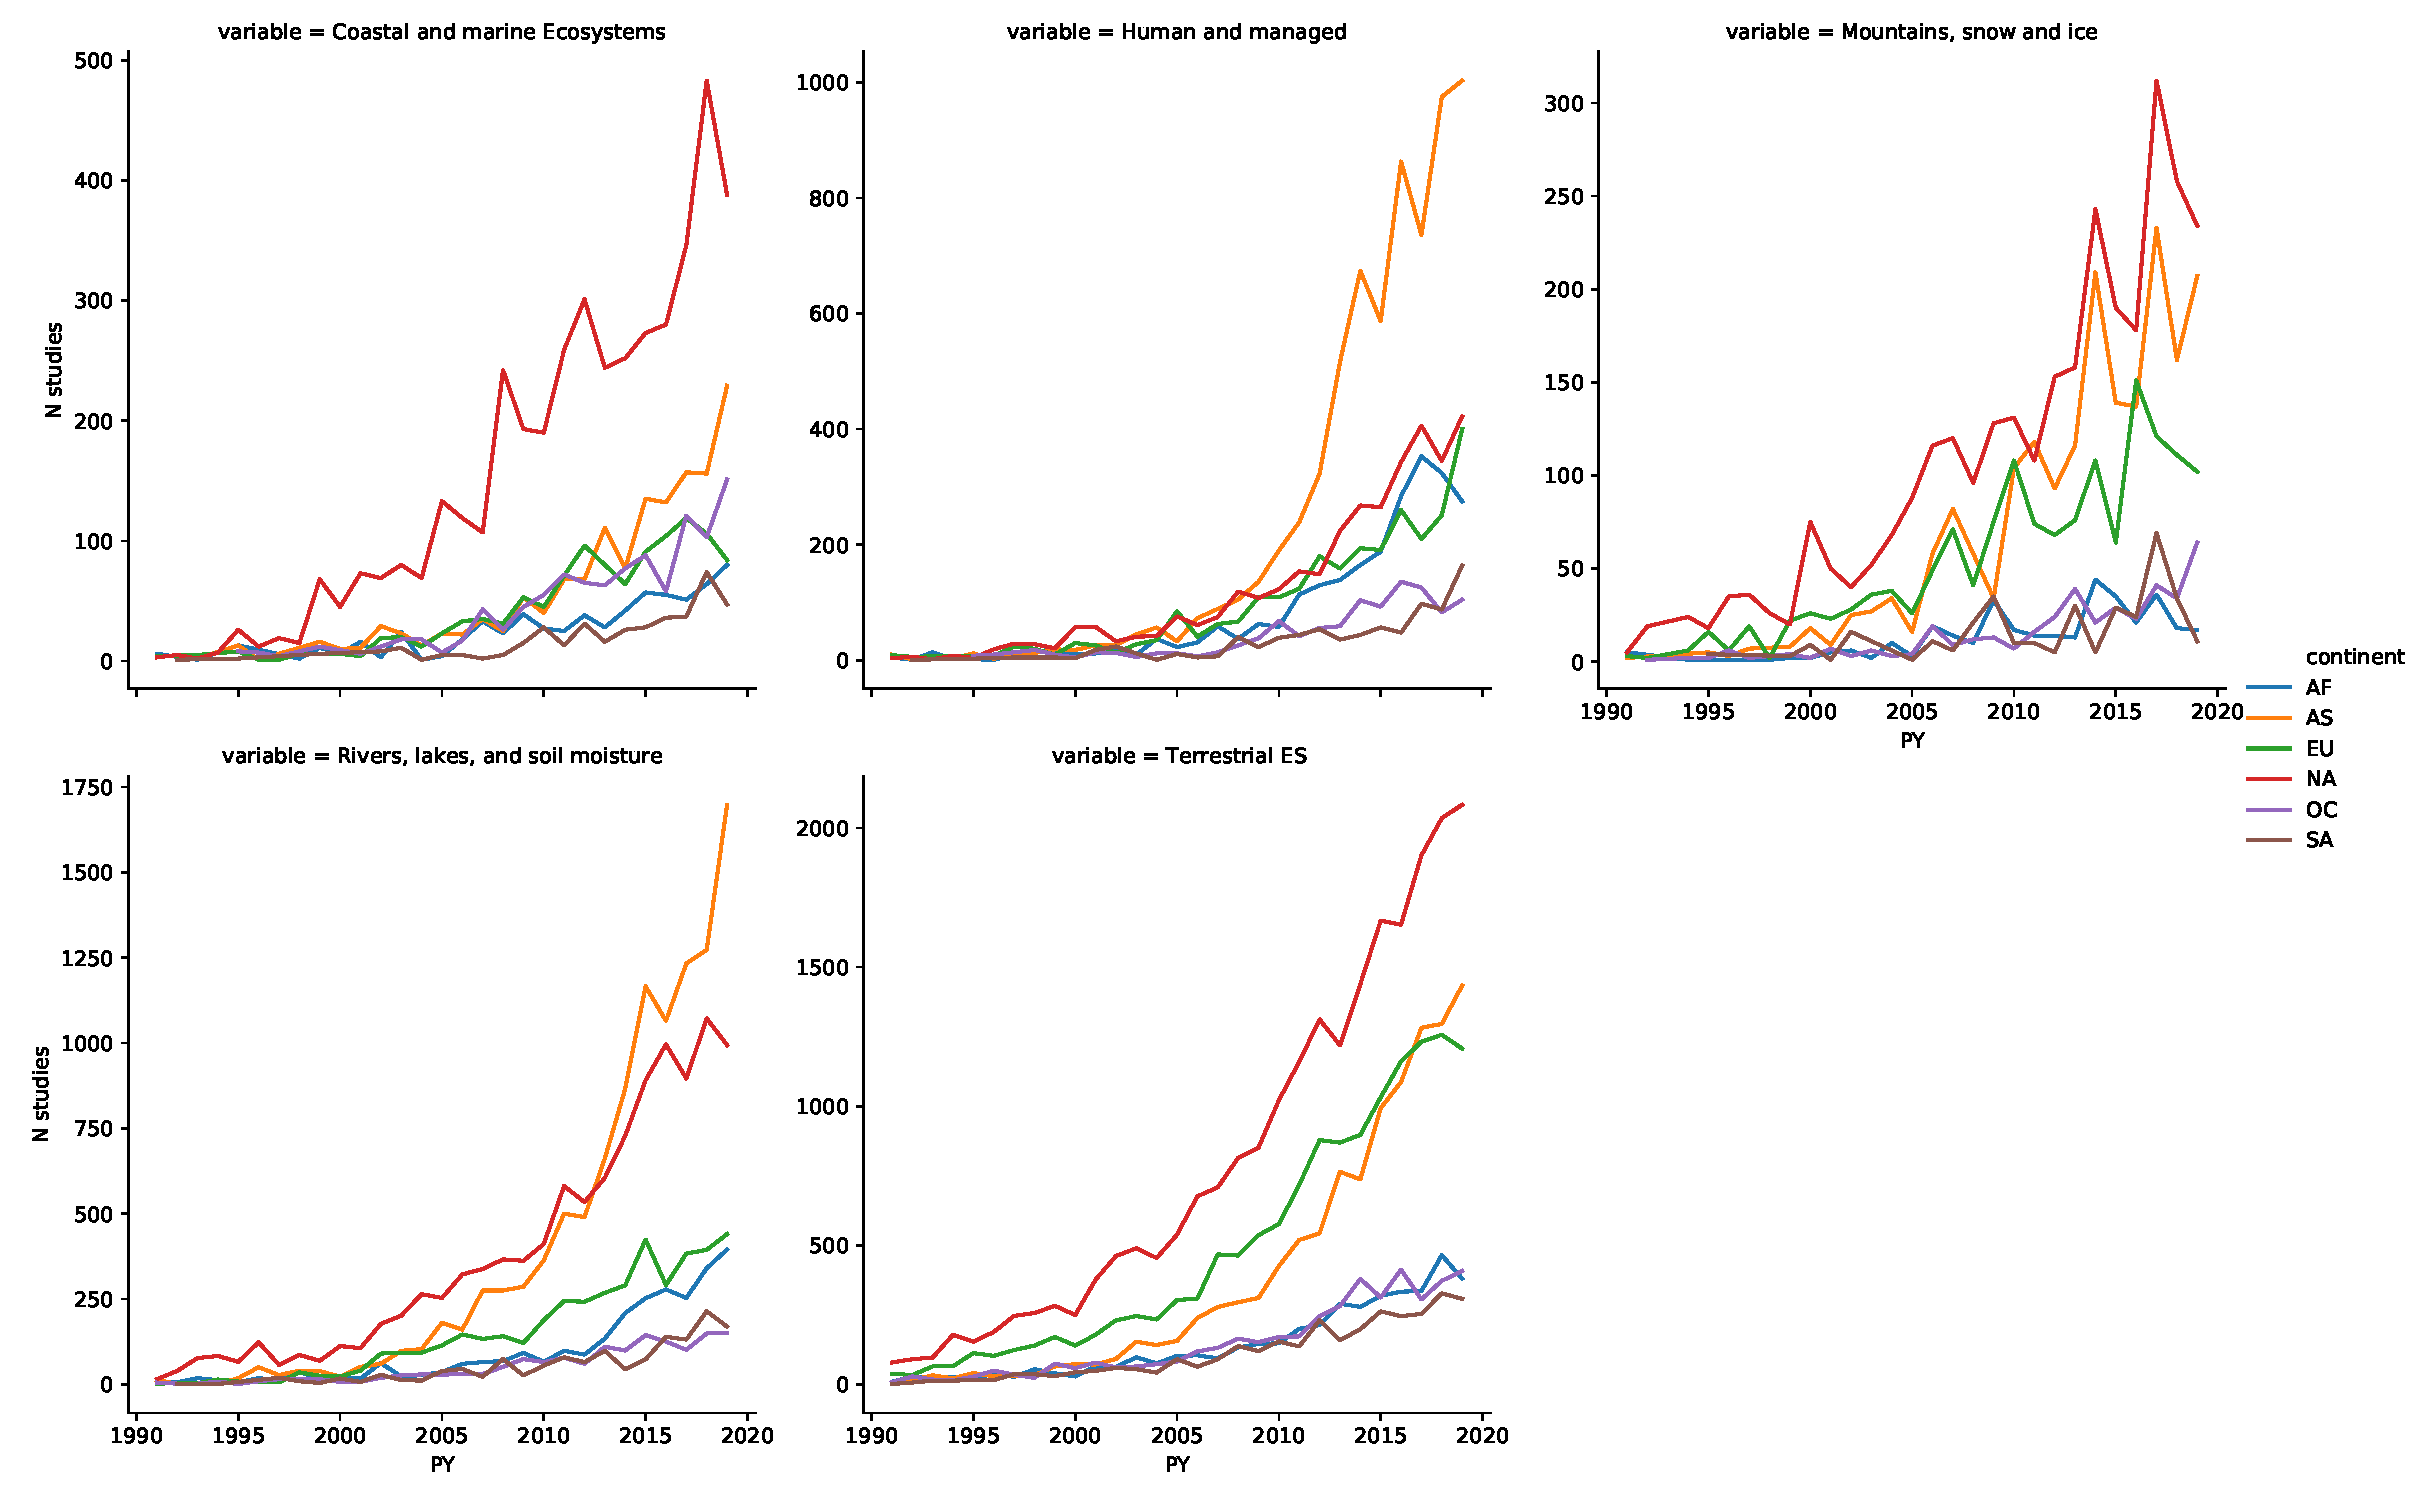
\includegraphics[width=\linewidth]{../plots/literature_distribution/PY_continent_impact.pdf}}
	
\end{column}
\end{columns}

\end{frame}



\end{document}